\subsection{Conversão de Intervalo}

Converte o intervalo de intensidade da imagem de [0, 255] para [100, 200] linearmente.

\begin{figure}[H]
    \centering
    \begin{subfigure}{0.45\textwidth}
        \centering
        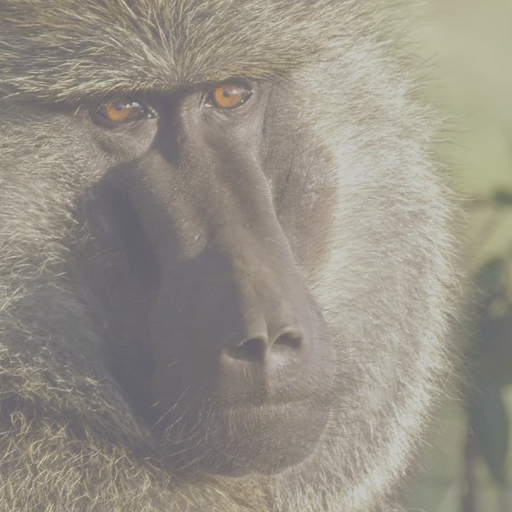
\includegraphics[width=6cm]{resultados/colorconv.png}
        \caption{\texttt{imagens/color.png}}
    \end{subfigure}%
    \begin{subfigure}{0.45\textwidth}
        \centering
        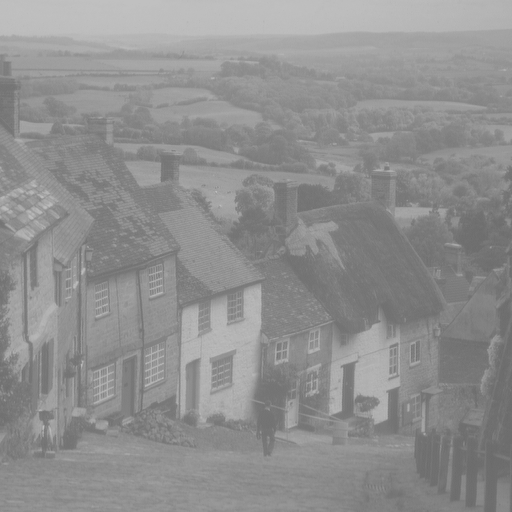
\includegraphics[width=6cm]{resultados/cityconv.png}
        \caption{\texttt{imagens/city.png}}
        \label{fig:res:4}
    \end{subfigure}

    \caption{Intervalo de intensidade convertido.}
\end{figure}

\begin{listing}[H]
    \begin{minted}{python}
        def converter_intervalo(imagem):
            zmin, zmax = np.min(imagem), np.max(imagem)
            img = 100 * (image / 255) + 100
            return img.astype(np.uint8)
    \end{minted}

    \caption{Comando \texttt{conv.intervalo}}
\end{listing}
